\documentclass[class=../report, crop=false]{standalone}
\usepackage{graphicx}

\begin{document}

\section{Final Prototype and Competition Results}

We developed our final \gls{prototype} from the best concept selected in the WDM.
We combined a mechanical gear transmission with an electronic braking system.
However, we scored poorly in competition because we ineffectively implemented reliability in our design.

\subsection{Final Prototype}

Our final prototype (Figure \ref{fig:finalmech}) uses two motors to power a single variable gear train.
The chassis is low to the ground and contains all the mechanical components.

\begin{figure}[H]
	\centering
	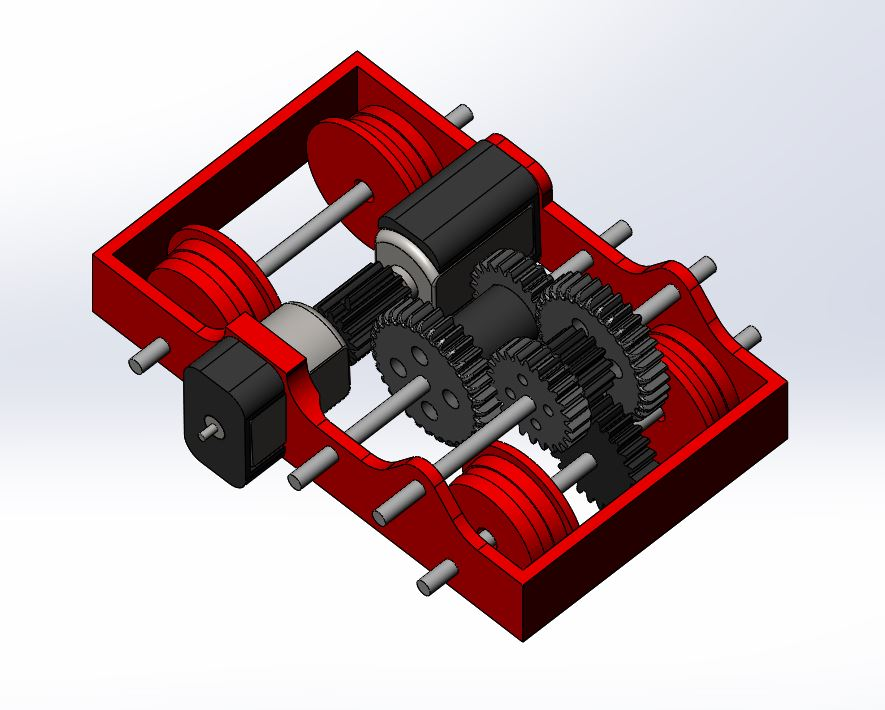
\includegraphics[width=0.8\textwidth]{../res/img/finalmech}
	\caption{Mechanical System of Final Prototype}
	\label{fig:finalmech}
\end{figure}

The circuitry is mounted above the mechanical systems.
A photoresistor detects the number of track ties the train passes over.
After a certain number, the \gls{arduino} reverses the polarity on the motor, causing the train to brake.
Once acceleration reaches zero, a gyroscope sensor tells the Arduino to stop braking.
The circuitry implementation is availible in Appendix \ref{app:finaldetails}: \nameref{app:finaldetails} Figures \ref{app/fig:circuit}--\ref{app/fig:finalprototypecircuitry}.

Our final prototype can reach a top speed of 1.56m/s; this value was much higher than we desired due to underestimations of the gear ratio needed for competition.
The train can climb 31$^{\circ}$ inclines; however, the locomotive is incapable of hauling more than an empty cargo cart.
We use 3 batteries to power the train.
The locomotive costs \$80.43\footnotemark, where the primary cost is the \gls{arduino}.
\footnotetext{See Appendix \ref{app:bom}: \nameref{app:bom}}

\subsection{Competition Performance}

We scored 17th place in the competition with 14.9 points.
Our train did not have enough torque to climb the 45$^{\circ}$ hill.
However, the majority of points were lost because our train could not complete the track in rounds two through five.
In the second round, we underestimated the locomotive’s height and it was incapable of passing through the first tunnel.
The braking system we used was not reliable and our train could not slow down for turns if it did not engage, which occured in our retrial of round two.
The system also propelled our train backwards when the proximity sensor mistakenly counted track ties in round three.
The circuitry connections were loose and this resulted in the train failing to start in round four.
\end{document}
